\section{Conclusion}
\label{ch:conclusion} % For easy referencing
In this final year project, We have explored the implementation and development of mesh networks within the challenging environment of a forest. Through:
\begin{enumerate}
    \item The wireless commutation environment 
    \item The desired characteristics of the sensors
    \item The available electronic devices for this limitation
    \item The limited hardware available
    \item The  fundamental software needed
    \item The Setup of the software
    \item The examination of the programming software needed
    \item The test before the writing of any code 
    \item The discussion of how to record data
    \item The Limitations
\end{enumerate}
\subsection{Key Contributions}

This project has contributed significantly to the understanding of the process of developing mesh networks in forest settings by:

\begin{itemize}
    \item \textbf{Developing a Model:} In this we used serial communication to test the nature of  which the network will send/ receive data from the network 
    \item \textbf{Addressing Challenges:} in a line of sight environment the sending and receiving of images is a hard task due to  how large the file is byte by byte
    \item \textbf{Performance Evaluation:} every method eventually worked via serial but image files had the  most problems
    \item \textbf{Practical Implications:} Schedule the sending  and  receiving  of data we can use this to extract the sensor data
    \item \textbf{Familiarity with different tools:} This project forces the project implementation to use the terminal in Linux, bash, In Linux the concept of Dev files are files where the port can be defined for example port 80 on the window would be \textcolor{yellow}{/dev/tty80}, also the addition of tools like ssh which allowed remote connection to the Pi board, batch files used to make these connections easier, A stronger familiarly with git was gained due to the keeping the project version controlled, A display of further knowledge of python was gain due to  project such as  using virtual environments and  how to properly structure OPP program, An understanding of  TDD for coding projects was gained where the implementor is forced to  use these methods
\end{itemize}
\section{Sources of Error}
In this section, the following will be discussed:
\begin{enumerate}
    \item Radio module
    \item MCP3008
    \item Time management
    \item Lack of knowledge of Linux OS
    \item Camera
    \item Lack of hat for sensors
\end{enumerate}
\subsection{Radio Module}
This section will discuss the problems noticed while working on this:
\begin{enumerate}
    \item When trying to look for radio modules for the MM2 Series 900 MHz this part couldn't be ordered due to the vendor only accepting business customers this cost 4 weeks of research to look for another module
    \item Once the appropriate modules were after looking and noticing that the documentation was very poor it did help as well.
    \item One avenue not expected of this was enabling the serial. So once we enable via sudo raspi-config, and use the code from this \href{https://github.com/sbcshop/Lora-HAT-for-Raspberry-Pi}{link} (use lora\_receiver.py and lora\_transmitter.py) when we get the following error:

    \begin{figure}[h!]
        \centering
        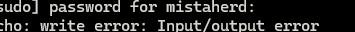
\includegraphics[width=0.5\linewidth]{Images/write_issue_linux_ser.png}
        \caption{Issue when trying to write to serial }
        \label{Issue when trying to write to serial}
    \end{figure}
    This issue took a lot of time to fix a simple chmod rw operation will fix the issue which should be indicated in the documentation but there isn't.
    \item After getting a working demo on all use cases of the module the image file caused the most issues this was due to the nature of how large the large data in an image file further research should have been put into how an image is sent across a communication channel.
    \item The lack of documentation meant time was spent looking at the components on board and finding how they worked. 
\end{enumerate}
\subsection{MCP3008}
In this section the Errors that occurred with this module are the following:
\begin{enumerate}
    \item When it came to ordering this part, There were issues with the venter so another ADC had to be chosen this caused another few weeks to go by.
\end{enumerate}
\subsection{Lack of knowledge of Linux os}
This section will discuss the errors that occurred theses are the following:
\begin{enumerate}
    \item Since the lack of experience with Linux is evident  this led to time spent learning about certain commands that will help with the project concepts such as  piping  commands nmap where  foreign before this project a lot of time was spent learning the best tools for this project
\end{enumerate}
\subsection{Camera}
This Section will discuss the errors that occurred with this module these are the following:
\begin{enumerate}
    \item When using the python file "camera.py" this wouldn't comply due to how the old library is no longer supported this costs around 2 weeks due to finding different forms and tracking the right library down eventually. the decision was made to make a bash command  to run the camera
\end{enumerate}
\subsection{Lack of hat for sensors}
This Section will discuss the issues of this which are  the following:
\begin{enumerate}
    \item When wiring up all the sensors it took several minutes to wire the devices up which led to miss wiring the temp sensor which blew  leading to an order for a replacement to be made
    \item This issue along with the could have led to  the code being simpler in nature them what is present in the repository
\end{enumerate}
\section{Future Work}

While this project hasn't achieved its core objectives, several avenues for future research and development remain open:

\begin{itemize}
    \item \textbf{Sockets:} The project could have ventured into socket programming, A socket is an endpoint of a two-way communication link between two programs running on the network. we picked serial communication for testing but this is where the main server and client can defined.
    \item \textbf{Helpful Tools:}  Linux has a wide range of networking tools such as:
    \begin{itemize}
        \item\textbf{Nmap} is a network scanner designed to discover hosts and services on a computer network. It sends packets and analyzes the responses to gather information 
        \item \textbf{ifconfig} Which provides extensive control over interfaces, addresses and routes
        \item \textbf{traceroute} Traces the route packets take to reach a destination
        \item \textbf{route} Displays or manipulates the kernel's IP routing table
        \item \textbf{arp} Displays and manages the Address Resolution Protocol (ARP) cache, which maps IP addresses to MAC addresses
        \item \textbf{tcpdump} Captures and analyzes network traffic, useful for diagnosing network issues.
        \item \textbf{iftop} Displays a real-time bandwidth monitor for network interfaces.
    \end{itemize} 
    \item \textbf{Energy Efficiency:} Investigate further what can be done to make  our system more energy effective i.e piplineing the sensor data
    \item \textbf{Security:} Investigate how to make our data secure via RSA and different protocols
    \item \textbf{PCB board :} After testing the board one problem was wiring up the sensor a potential for making a custom  Pi hat that will provide an easy way of connecting  our sensor 
 
   
\end{itemize}
\newpage
\subsection{Final Remarks}
The deployment of mesh networks in forest environments holds immense promise. The work provided here doesn't outline how to achieve this but can be viewed as a method to achieving  this nature